%%%%%%%%%%%%%%%%%%%%%%%%%%%%%%%%%%%%%%%%%
% NIWeek 2014 Poster by T. Reveyrand
% www.microwave.fr
% http://www.microwave.fr/LaTeX.html
% ---------------------------------------
%
% Original template created by:
% Brian Amberg (baposter@brian-amberg.de)
%
% This template has been downloaded from:
% http://www.LaTeXTemplates.com
%
% License:
% CC BY-NC-SA 3.0 (http://creativecommons.org/licenses/by-nc-sa/3.0/)
%
%%%%%%%%%%%%%%%%%%%%%%%%%%%%%%%%%%%%%%%%%

%----------------------------------------------------------------------------------------
%   PACKAGES AND OTHER DOCUMENT CONFIGURATIONS
%----------------------------------------------------------------------------------------

\documentclass[a0paper,landscape]{baposter}

\usepackage[font=small,labelfont=bf]{caption} % Required for specifying captions to tables and figures
\usepackage{booktabs} % Horizontal rules in tables
\usepackage{relsize} % Used for making text smaller in some places

\usepackage{amsmath,amsfonts,amssymb,amsthm} % Math packages
\usepackage{eqparbox}

\usepackage{textcomp}

\usepackage{caption}
\usepackage{subcaption}
\usepackage{graphicx}
\usepackage{listings}
\usepackage{mathtools}
\usepackage[percent]{overpic}


\usepackage{multirow}
%\usepackage{verbatimbox}
%\usepackage{hyperref}

%\usepackage{pgf}

\usepackage[utf8]{inputenc}
\usetikzlibrary{shapes,arrows}
\usepackage{tikz}
\usetikzlibrary{automata,positioning}

\usepackage{multicol}

\usepackage{hyperref}

\usepackage[font=small,labelfont=bf]{caption}

\usepackage{makecell}
\usepackage{enumitem}

\renewcommand\theadalign{bc}
\renewcommand\theadfont{\bfseries}
\renewcommand\theadgape{\Gape[4pt]}
\renewcommand\cellgape{\Gape[4pt]}


\setlist[itemize]{leftmargin=*}

\graphicspath{{figures/}} % Directory in which figures are stored

 \definecolor{bordercol}{RGB}{40,40,40} % Border color of content boxes
 \definecolor{headercol1}{RGB}{210,235,250} % Background color for the header in the content boxes (left side)
 \definecolor{headercol2}{RGB}{210,235,250} % Background color for the header in the content boxes (right side)
 \definecolor{headerfontcol}{RGB}{0,0,0} % Text color for the header text in the content boxes
 \definecolor{boxcolor}{RGB}{240,255,255} % Background color for the content in the content boxes

\tikzset{
    state/.style={
           ellipse,
           draw=black, thin,
           minimum height=0.5cm,
           minimum width=0.6cm,
           text centered,
           font=\scriptsize
           },
    horiz/.style={
           % font=\tiny,
           inner sep=3pt,
           font=\bf

           } ,
    point/.style={
           circle,
           minimum width = 5pt,
           fill
           }
}

\begin{document}

\setlength{\fboxsep}{0pt}

\background{ % Set the background to an image (background.pdf)
\begin{tikzpicture}[remember picture,overlay]
\draw (current page.north west)+(-2em,2em) node[anchor=north west]
{\includegraphics[height=1.1\textheight]{background}};
\end{tikzpicture}
}

\begin{poster}{
grid=false,
columns=12, % because reasons
borderColor=bordercol, % Border color of content boxes
headerColorOne=headercol1, % Background color for the header in the content boxes (left side)
headerColorTwo=headercol2, % Background color for the header in the content boxes (right side)
headerFontColor=headerfontcol, % Text color for the header text in the content boxes
boxColorOne=boxcolor, % Background color for the content in the content boxes
headershape=rectangle, % Specify the rounded corner in the content box headers
headerfont=\Large\sf\bf, % Font modifiers for the text in the content box headers
textborder=none,
background=none,
headerborder=none, % Change to closed for a line under the content box headers
boxshade=plain
}
{
\includegraphics[width=4cm]{jr.png}}
%
%----------------------------------------------------------------------------------------
%   TITLE AND AUTHOR NAME
%----------------------------------------------------------------------------------------
%
{\bf \huge{Context-Free Path Querying with All-Path Semantics by Matrix Multiplication} }
%\\  \Large \it Context-free grammars and neural networks for secondary structure} % Poster title
{\vspace{0.6em} \smaller \textbf{Rustam Azimov} \\  % Author names
\smaller \it {JetBrains Research, Saint Petersburg University, Russia } \\ % Author email addresses
\smaller  {Rustam.Azimov@jetbrains.com}}
{
\includegraphics[width=2.5cm]{SPbGU_Logo.png}} % University/lab logo


%----------------------------------------------------------------------------------------
%   INTRODUCTION
%----------------------------------------------------------------------------------------
\begin{posterbox}[name=CFPQ,column=0,row=0, span=4]{All-Path CFPQ}

  Find all paths which satisfy constraints in form of a formal language $L=\{a^n b^n \mid n > 0\}$
    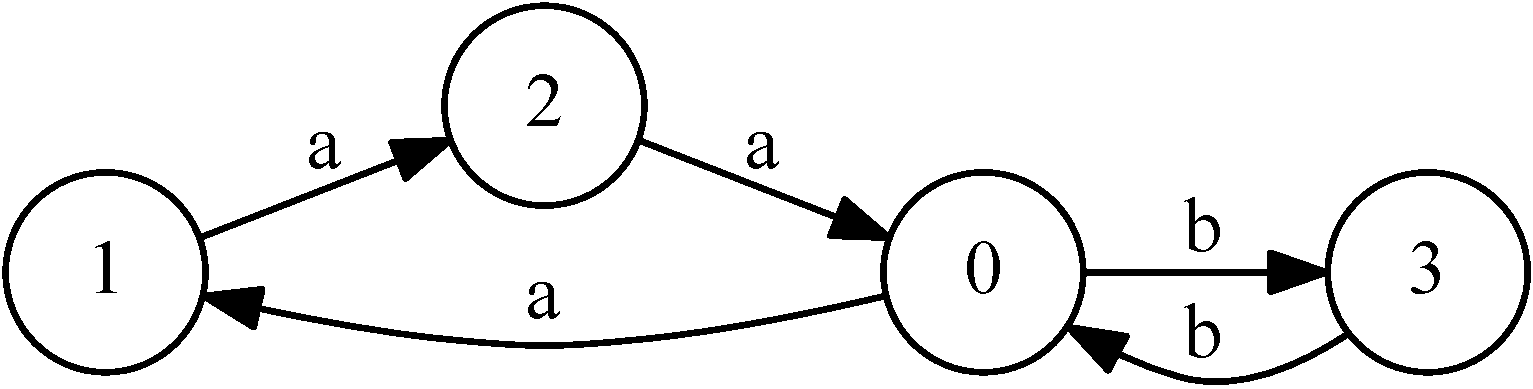
\includegraphics[width=7cm]{example_graph_transparent.png}

    Query = grammar for $L$: $S  \rightarrow a  \ b \ | \ a \ S \ b  \\$

  In some cases we want to find all data dependencies, for example in static code analysis when
  searching for vulnerabilities

\end{posterbox}

\headerbox {Matrix-Based Algorithm~\cite{all-path2021}}
{name=matrices,column=0,span=6, row=2, below=CFPQ}%,bottomaligned=sol2}
{
	
	\begin{itemize}
		\item We store the additional information about the paths found as the sets of the intermediate vertices
		\item We introduce the following matrix multiplication operation
		\item $T^A \odot T^B = T^C$ where $T^C_{i,j} = \bigcup^{n}_{k = 1} (T^A_{i,k} \otimes T^B_{k,j})$ and   $T^A_{i,k} \otimes T^B_{k,j} = \begin{cases} \{k\}, & \mbox{if } T^A_{i,k} \neq \emptyset \wedge T^B_{k,j} \neq \emptyset \\ \emptyset, & \mbox{otherwise} \end{cases}$
	\end{itemize}

}

\headerbox {Results}{name=results,column=4,row=0, span=4, bottomaligned=CFPQ}{
\begin{itemize}
  \item We provide the matrix-based algorithm for CFPQ with all-path query semantics
  \item We implement the provided algorithm using the GraphBLAS API
  \item The proposed matrix-based solution for all-path query semantics compared to the Kronecker product-based solution consumes more memory, but allows one to extract paths significantly faster 
\end{itemize}
}

\headerbox {Future Research}{name=answers,column=8,row=0, span=4, bottomaligned=results}{

\begin{itemize}
  \item We plan to obtain GPU-based and distributed implementations
  \item Try to update the query results dynamically when data changes
  \item We plan to provide the multiple-source
  modifications for all linear algebra-based CFPQ algorithms
  \item Find new applications that required CFPQ
\end{itemize}

}


\headerbox {Path Extraction}
{name=impl,column=6,span=6, row=2, below=results,bottomaligned=matrices}
{
\begin{itemize}
	\item After constructing a set of matrices with sets of intermediate vertices, we can extract all required paths $i\pi j$ for every vertex pair $i, j$ if such paths exist
	\item It is	assumed that the sets of paths are computed lazily, to ensure the	termination in case of an infinite number of paths
	
\end{itemize}
}

%\setlength{\tabcolsep}{5pt}
%\headerbox{Linear Algebra-Based CFPQ Implementations }{name=rdfs,span=12,column=0,row=3,below=matrices}{
%	\vspace{0.05cm}
%	\begin{minipage}[t]{0.48\textwidth}
%		\begin{itemize}
%			\item We use the GraphBLAS API and sparse matrix representation
%			\item Our implemenationts are CPU-based
%			\item Implementation of the Kronecker product-based algorithm:
%			\begin{itemize}
%				\item $\textbf{Tns}$ --- our Python implementation for all-path query semantics		
%			\end{itemize}
%		\end{itemize}
%	\end{minipage}
%	~
%	\begin{minipage}[t]{0.5\textwidth}
%		\begin{itemize}
%			\item Our matrix-based CFPQ implementations:
%			\begin{itemize}
%				\item $\textbf{MtxRel}$ --- relational query semantics, uses \textbf{pygraphblas} --- a Python wrapper around the GraphBLAS API
%				\item $\textbf{MtxSingle}$ --- single-path query semantics, utilizes \textbf{pygraphblas}
%				\item $\textbf{MtxAll}$ --- all-path query semantics, operating over AllPathIndex
%			\end{itemize}
%		\end{itemize}
%	\end{minipage}
%}


\headerbox{CFPQ Evaluation with Relational, Single-Path and All-Path Query Semantics}{name=scaling,span=12,column=0,row=2,below=matrices}{
\vspace{0.05cm}
%\begin{table}[h]
%\rowcolors{1}{}{red}
%\begin{center}
\begin{minipage}[t]{0.5\textwidth}
%\vspace{-4.5cm}
		\begin{tabular}{|l|l|l|l|l|l|l|l|l|l|l|}
			\hline
			\multicolumn{1}{|c|}{\multirow{2}{*}{Graph}} & \multicolumn{1}{c|}{\multirow{2}{*}{\#V}} & \multicolumn{1}{c|}{\multirow{2}{*}{\#E}} &  \multicolumn{2}{c|}{MtxRel} & \multicolumn{2}{c|}{MtxSingle} & \multicolumn{2}{c|}{MtxAll} & \multicolumn{2}{c|}{Tns} \\ \cline{4-11} 
			\multicolumn{1}{|c|}{}                       & \multicolumn{1}{c|}{}                     & \multicolumn{1}{c|}{}                     & Time         & Mem          & Time        & Mem        & Time           & Mem           & Time         & Mem    \\ \hline
			%pathways                                     & 6 238                                     & 18 598 & 0.01         & 140  & 0.01           & 671 & 0.01         & 49           & 0.01        & 122               \\ \hline
			%go-hierarchy                                 & 45 007                                    & 980 218                                   & 0.09         & 255 & 0.84           & 671 & 0.35        & 195        & 0.24        & 252                             \\ \hline
			%enzyme                                       & 48 815                                    & 109 695                                   & 0.01         & 181 & 0.01           & 217 & 0.02         & 61           & 0.02        & 132                            \\ \hline
			eclass\_514en                                & 239 111                                   & 523 727                                   & 0.06         & 181 & 0.16           & 216    & 0.22         & 126          & 0.27        & 193                         \\ \hline
			go                                           & 272 770                                   & 534 311                                   & 0.94         & 246  & 0.93           & 217  & 1.13         & 990          & 1.27        & 243                          \\ \hline
			%geospecies                                   & 450 609                                   & 2 311 461                   & 0.01         & 248 & 0.01           & 2251            & 0.34         & 156          & 0.01        & 196              \\ \hline
			geospecies & 450 609                                   & 2 311 461 & 7.48         & 7645     & 15.54          & 22941 & 32.06        & 44235        & 26.32       & 19537 \\ \hline
			taxonomy                                     & 5 728 398                                 & 14 922 125                            & 0.72         & 1175      & 1.15           & 2250    & 3.84        & 1507        & 3.56        & 1776                   \\ \hline
		\end{tabular}

\end{minipage}~
\begin{minipage}[t]{0.3\textwidth}
\vspace{-0.8cm}
\begin{overpic}[width=0.8\textwidth]{plots/go_10_all_matrixall_tensor.pdf}
    \put (15,75) {{Average path extraction time for \textbf{go}}}
  \end{overpic}
%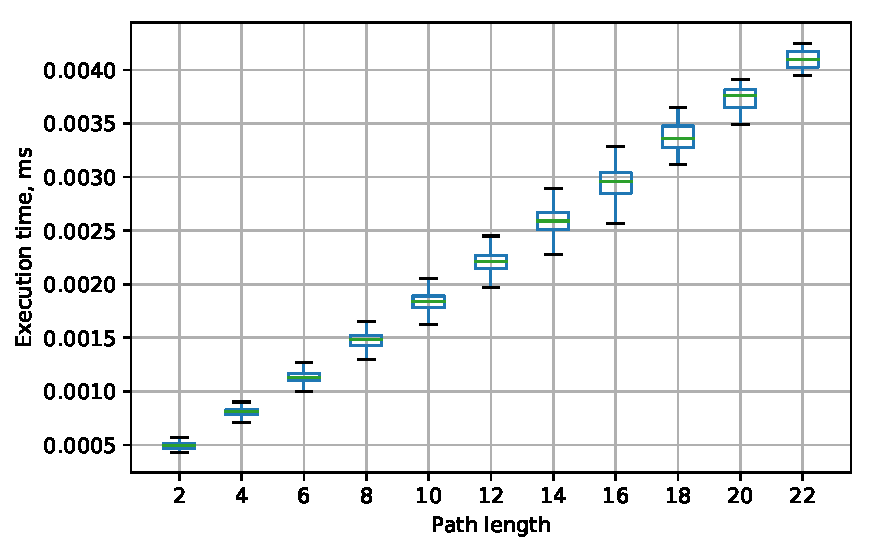
\includegraphics[width=0.95\textwidth]{plots/G1_go.pdf}
\end{minipage}~
\begin{minipage}[t]{0.18\textwidth}

\begin{itemize}
	\item \textbf{MtxAll} constructs index up to 2-3 times slower and consumes more memory than \textbf{MtxSingle}
	\item If we must extract paths many times for a once constructed
	index then \textbf{MtxAll} is  preferable than \textbf{Tns}
\end{itemize}
\end{minipage}~

\begin{minipage}[t]{0.5\textwidth}
	\vspace{-2.5cm}
	\begin{itemize}
		\item Time in seconds and memory is measured in megabytes
		\item  Graph: real-world ontologies (RDFs), query: same-generation query
		\item Example of a grammar: $S \to \textit{scor} \ S \ \textit{sco} \ | \ \textit{tr} \ S \ \textit{t} \ | \ \textit{scor} \ \textit{sco} \ | \ \textit{tr} \ \textit{t}$
	\end{itemize}
\end{minipage}
}



\headerbox {\smaller{Contact Us}}{name=contact,column=0,span=5,below=scaling}{
\scriptsize
\begin{minipage}[t]{0.65\textwidth}
  \vspace{-2.5cm}
\begin{itemize}
  \item Semyon Grigorev: \href{mailto:s.v.grigoriev@spbu.ru}{s.v.grigoriev@spbu.ru}
  \item Rustam Azimov:\href{mailto:Rustam.Azimov@jetbrains.com}{Rustam.Azimov@jetbrains.com}
  \item Ilya Epelbaum: \href{mailto:iliyepelbaun@gmail.com}{iliyepelbaun@gmail.com}
\end{itemize}


\end{minipage}
~
\begin{minipage}[t]{3cm}

\includegraphics[width=2.8cm]{qr-research-jetbra.pdf}
\vspace{0.7cm}
\end{minipage}
%\vspace{1cm}
{\scriptsize
%Both dataset and implementations are available on GitHub
\vspace{-1cm}
\begin{itemize}
	\item Dataset:
	\url{https://github.com/JetBrains-Research/CFPQ_Data}
	\item Implementations:
	\url{https://github.com/JetBrains-Research/CFPQ_PyAlgo}
\end{itemize}
}

}



\headerbox{\smaller{References}}{name=references,column=5,span=7,below=scaling}{

    \scriptsize % Reduce the font size in this block
    \renewcommand{\section}[2]{\vskip 0.05em} % Get rid of the default "References" section title
    \nocite{*} % Insert publications even if they are not cited in the poster
    \bibliographystyle{unsrt}
    \bibliographystyle{IEEEtran}
    \bibliography{biblio} % Use biblio.bib as the bibliography file
}

%\headerbox {\smaller{Acknowledgments}}{name=ack,column=5,span=7,below=references}{
%\small
%The research was supported by the Russian Science Foundation,
%grant number 18-11-00100
%}

%{\hspace{5pt}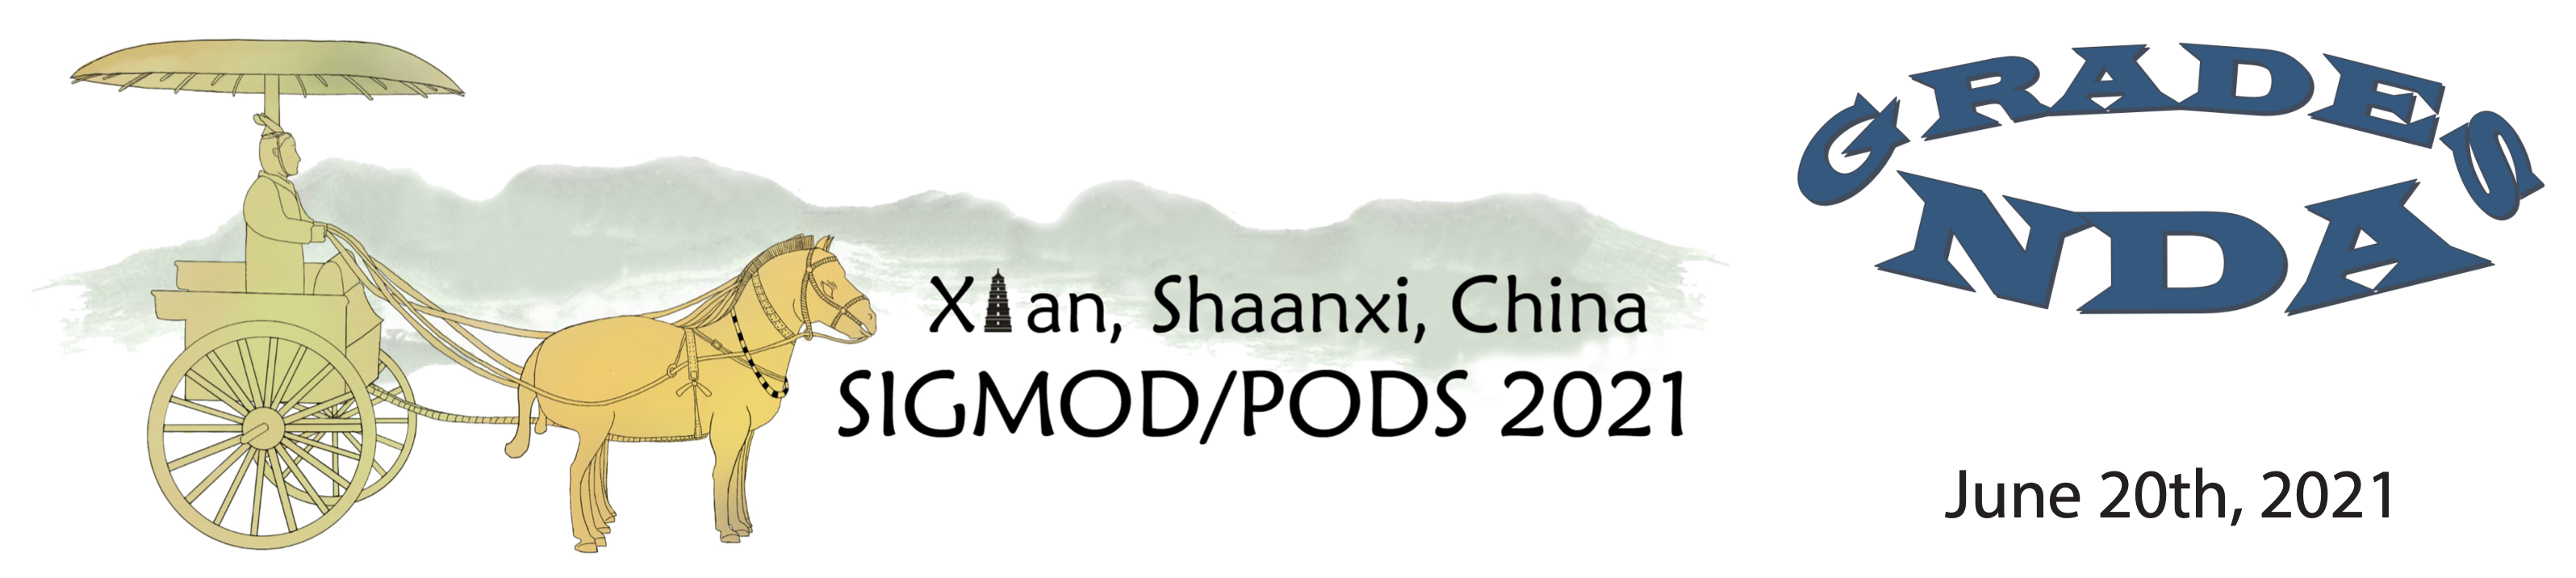
\includegraphics[width=0.4\textwidth]{logo2021.png}}


\end{poster}


\end{document}
